% Prof. Dr. Ausberto S. Castro Vera
% UENF - CCT - LCMAT - Curso de Ci\^{e}ncia da Computa\c{c}\~{a}o
% Campos, RJ,  2023
% Disciplina: Paradigmas de Linguagens de Programa\c{c}\~{a}o
% Aluno: Mariana Cossetti Dalfior


\chapter{Ferramentas existentes e utilizadas}

Neste cap\'{\i}tulo serão apresentadas duas ferramentas que foram consultadas e utilizadas para realizar este livro, e usadas nas aplica\c{c}\~{o}es:

%%%=========================================================================================%%%
\section{PyCharm}
%%%=========================================================================================%%%

PyCharm \'{e} um IDE Python desenvolvido pela JetBrains. Ele foi projetado especificamente para Python e fornece muitos recursos que o tornam uma ferramenta poderosa para o desenvolvimento do Python. Atualmente, se encontra na vers\~{a}o 2023.1.

\begin{figure}[H]
	\begin{center}
		\caption{Ambiente inicial do PyCharm} \label{ambientepycharm}
		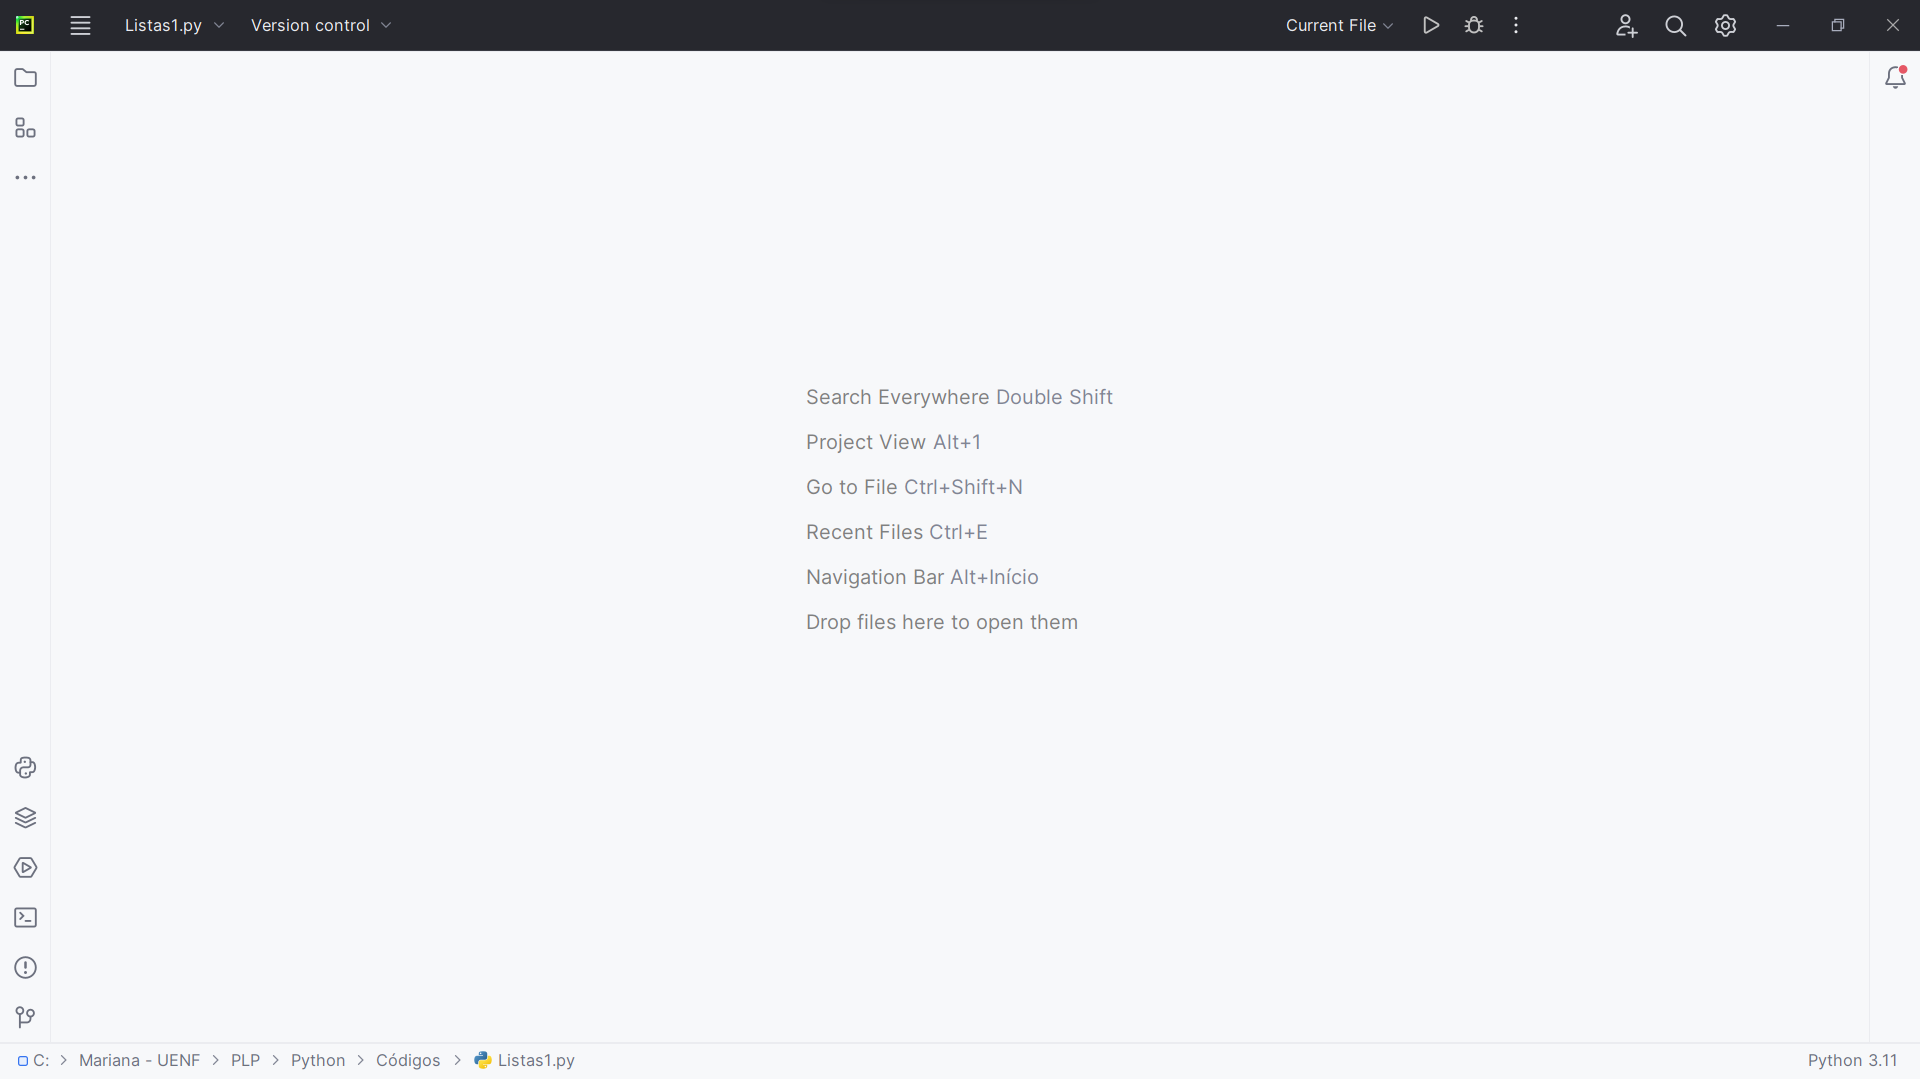
\includegraphics[width=12cm]{ambientepycharm} 
		\newline
		Fonte: Criado por Mariana Cossetti Dalfior
	\end{center}
\end{figure}

Uma das principais caracter\'{\i}sticas do PyCharm \'{e} seu sistema de depura\c{c}\~{a}o. Ele permite que voc\^{e} execute seu c\'{o}digo passo a passo e observe o estado de seu programa em cada etapa. Isso \'{e} muito \'{u}til para encontrar e corrigir bugs em seu c\'{o}digo. O PyCharm tamb\'{e}m possui um sistema de gerenciamento de projetos para organizar facilmente seu c\'{o}digo. Ele permite que voc\^{e} estruture seu projeto em diferentes m\'{o}dulos e pacotes, tornando seu c\'{o}digo mais f\'{a}cil de gerenciar e manter.

Al\'{e}m disso, o PyCharm oferece suporte a v\'{a}rios frameworks e bibliotecas Python, como Django, Flask e NumPy. Isso significa que voc\^{e} pode usar o PyCharm para desenvolver uma ampla variedade de aplicativos Python, de sites a aplicativos de ci\^{e}ncia de dados.  Para baix\'{a}-lo basta apenas acessar o site da ferramenta (\url{https://www.jetbrains.com/pt-br/pycharm/}).\newline

A seguir \'{e} poss\'{\i}vel observar o mesmo c\'{o}digo fonte \ref{fontelista} e o resultado \ref{resullista} do exemplo de c\'{o}digo em Python mostrado acima, por\'{e}m no IDE PyCharm, utilizado em \ref{cap3/3.2.1}:

\begin{figure}[H]
	\begin{center}
		\caption{C\'{o}digo fonte do exemplo do uso listas} \label{fontelista}
		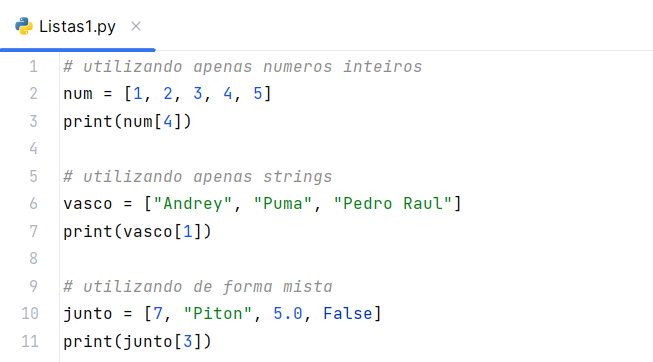
\includegraphics[width=12cm]{listas1pycharm} 
		\newline
		Fonte: Criado por Mariana Cossetti Dalfior
	\end{center}
\end{figure}

\begin{figure}[H]
	\begin{center}
		\caption{Resultado do c\'{o}digo fonte do exemplo do uso listas} \label{resullista}
		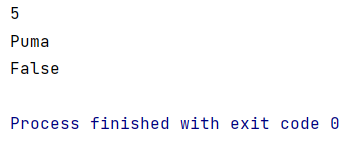
\includegraphics[width=9cm]{resullistas1pycharm} 
		\newline
		Fonte: Criado por Mariana Cossetti Dalfior
	\end{center}
\end{figure}

%%%=========================================================================================%%%
    \section{Visual Studio Code}
%%%=========================================================================================%%%
O Visual Studio Code, comumente conhecido como VS Code, \'{e} um editor de c\'{o}digo-fonte criado pela Microsoft que se tornou uma ferramenta essencial para muitos programadores Python. O software \'{e} leve, de c\'{o}digo aberto e gratuito e compat\'{\i}vel com muitas linguagens de programa\c{c}\~{a}o, incluindo Python. Atualmente, se encontra na vers\~{a}o 1.79 e \'{e} a que foi utilizada para a execu\c{c}\~{a}o dos c\'{o}digos deste livro. Al\'{e}m disso, pode ser utilizado em diversos sistemas operacionais como Windows, macOS e Linux. 

\begin{figure}[H]
	\begin{center}
		\caption{Ambiente inicial do Visual Studio Code} \label{ambientevs}
		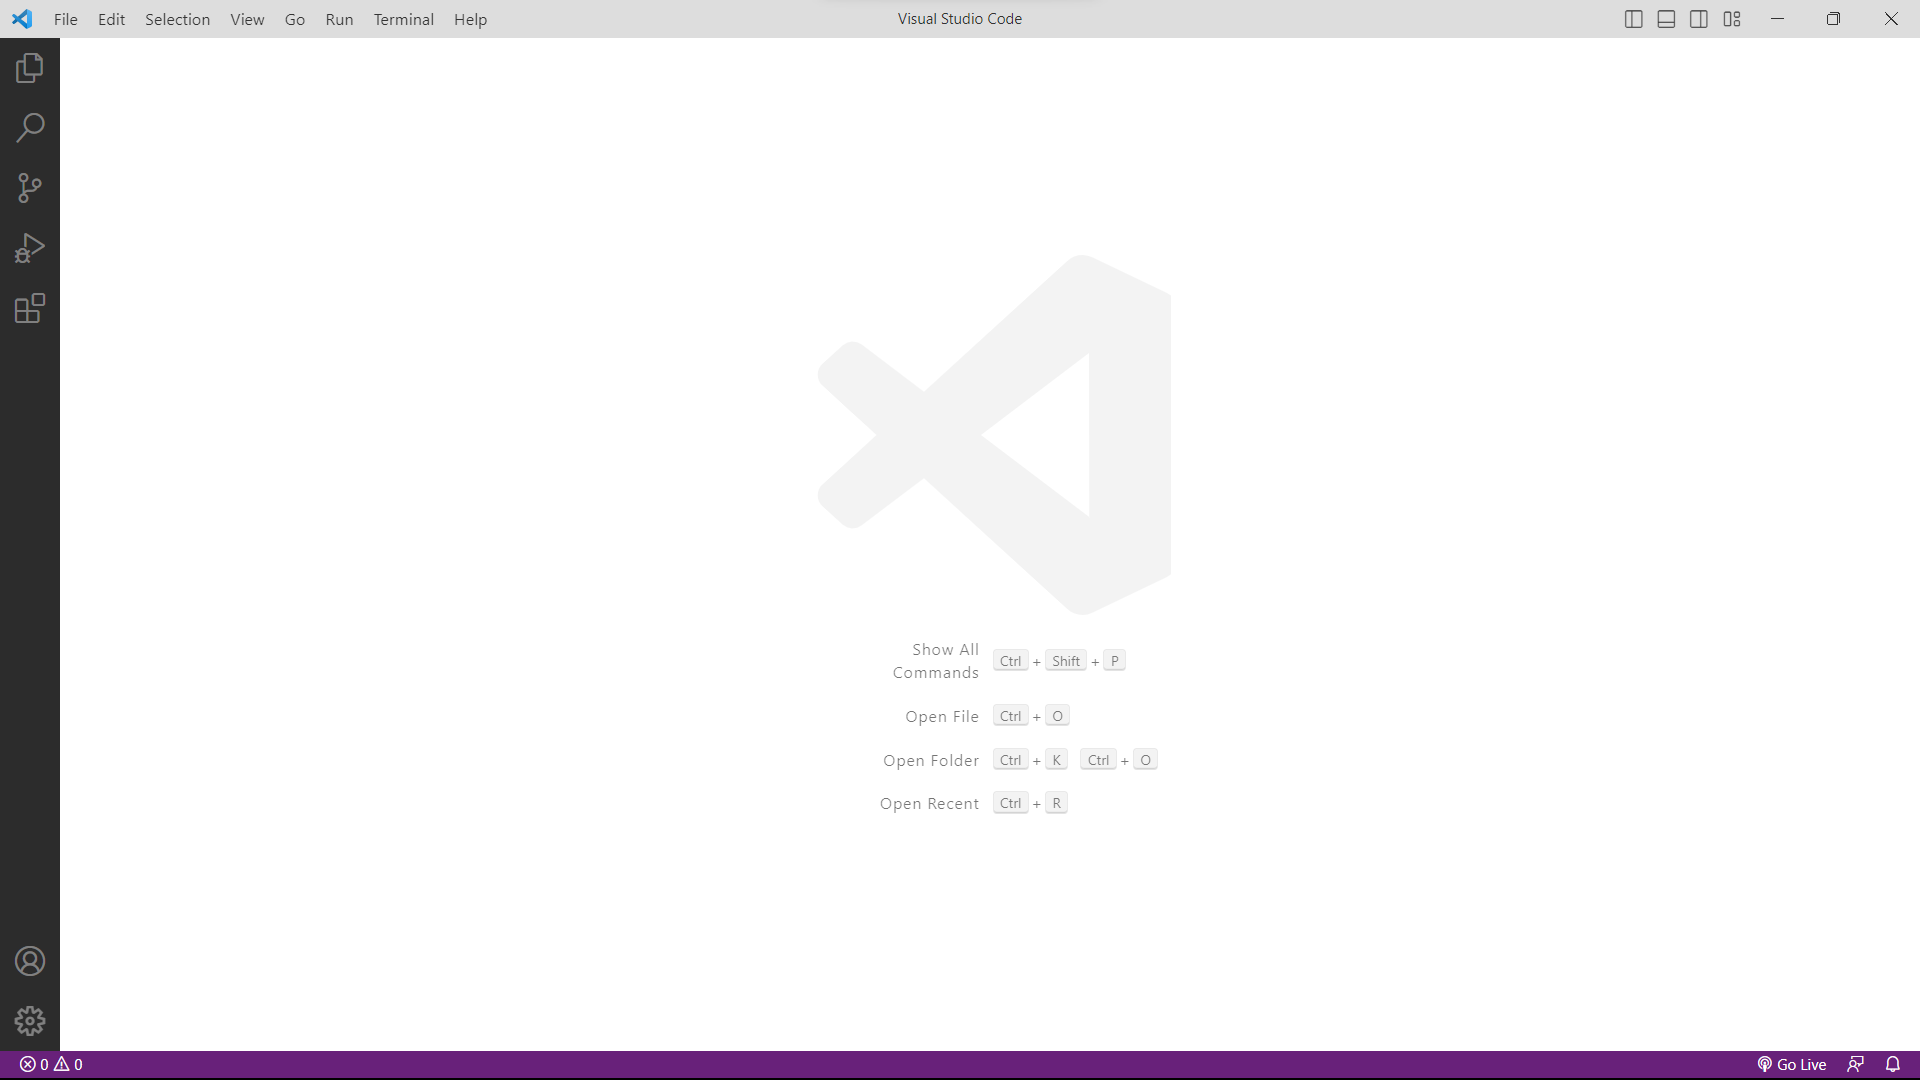
\includegraphics[width=12cm]{ambientevs} 
		\newline
		Fonte: Criado por Mariana Cossetti Dalfior
	\end{center}
\end{figure}

O VS Code fornece um conjunto de fun\c{c}\~{o}es que simplificam a programa\c{c}\~{a}o em Python. Possui um sistema de realce de sintaxe que torna o c\'{o}digo mais f\'{a}cil de ler e entender. Al\'{e}m disso, o VS Code possui um recurso de preenchimento autom\'{a}tico que sugere trechos de c\'{o}digo conforme o usu\'{a}rio digita, economizando tempo e minimizando a chance de erros de digita\c{c}\~{a}o.

Um recurso not\'{a}vel do VS Code \'{e} sua extensibilidade. Existem milhares de extens\~{o}es dispon\'{\i}veis que aumentam a funcionalidade do editor, como formata\c{c}\~{a}o autom\'{a}tica de c\'{o}digo, linting, depura\c{c}\~{a}o, teste de unidade e muito mais. Isso permite que voc\^{e} adapte o VS Code ao seu processo de desenvolvimento do Python. Para baix\'{a}-lo basta apenas acessar o site da ferramenta (\url{https://code.visualstudio.com/}). \newline

A seguir \'{e} poss\'{\i}vel observar o c\'{o}digo fonte \ref{fontelistas} e o resultado \ref{resullistas} do exemplo de c\'{o}digo em Python, utilizado em \ref{cap3/3.2.1}:

\begin{figure}[H]
	\begin{center}
		\caption{C\'{o}digo fonte do exemplo do uso listas} \label{fontelistas}
		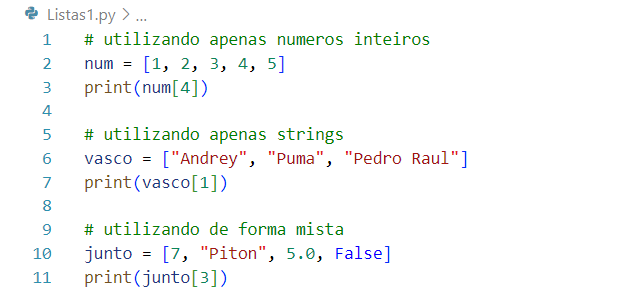
\includegraphics[width=12cm]{listas1} 
		\newline
		Fonte: Criado por Mariana Cossetti Dalfior
	\end{center}
\end{figure}

\begin{figure}[H]
	\begin{center}
		\caption{Resultado do c\'{o}digo fonte do exemplo do uso listas} \label{resullistas}
		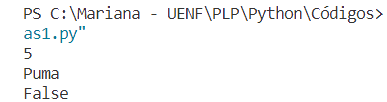
\includegraphics[width=9cm]{resullistas1} 
		\newline
		Fonte: Criado por Mariana Cossetti Dalfior
	\end{center}
\end{figure}
